Having explored existing data models and tested their limitations against several case studies from the Middle Ages, we propose a model with the entities and relationships represented in Figure \ref{fig:ProposedEntities}. To begin, we present all the entities we believe necessary for a data model tasked with organizing and delivering information about texts and traditions in Medieval literature, particularly texts about chivalric tales and legends. Then, we list all the attributes each entity features. Compared to the former, this latter section is more likely to need renegotiation based on the idiosyncratic qualities of different literary corpora.

\subsection{Entity relationships}

We start by simply introducing the entities' names and the nature of their relationships to one another. Subsequently, we present a technical schematic of the entities' relationships to one another. Figure \ref{fig:ProposedEntities} illustrates the entities and relationships in our proposed model.

\subsubsection{Intertextuality}

On the top level of Figure \ref{fig:ProposedEntities}, running from left to right, are the three abstract entities, \textit{Cycle}, \textit{Work}, and \textit{Text}, that manage information about intertextuality in our corpus. \textit{Works} and \textit{Cycles} can be nested together within the scope of a \textit{Cycle}, based on the \textit{Works'} narrative content; both entities have the attribute ``is part of,'' which points to a \textit{Cycle} entity. \textit{Works} can also be modeled on other works, as in the case of a new \textit{Work} compiling and reworking the episodes and characters from two or more pre-existing \textit{Works}. The data model also registers intertextuality amongst \textit{Texts}, which can be modeled on one another as translations, prosifications, abbreviations, elaborations, versifications, or other forms of adapting the expression (\textit{Text}) of a common \textit{Work}. The nature of a \textit{Text's} relationship to a model \textit{Text} can be inferred through differences and similarities in the two entities' attributes, such as their language and literary form.

\begin{figure}[ht]
    \begin{center}
        \tikzstyle{s} = [rectangle, rounded corners, minimum width=2cm, text width=2cm, minimum height=1cm, text centered, draw=black]
\tikzstyle{arrow} = [thick,->,>=stealth]
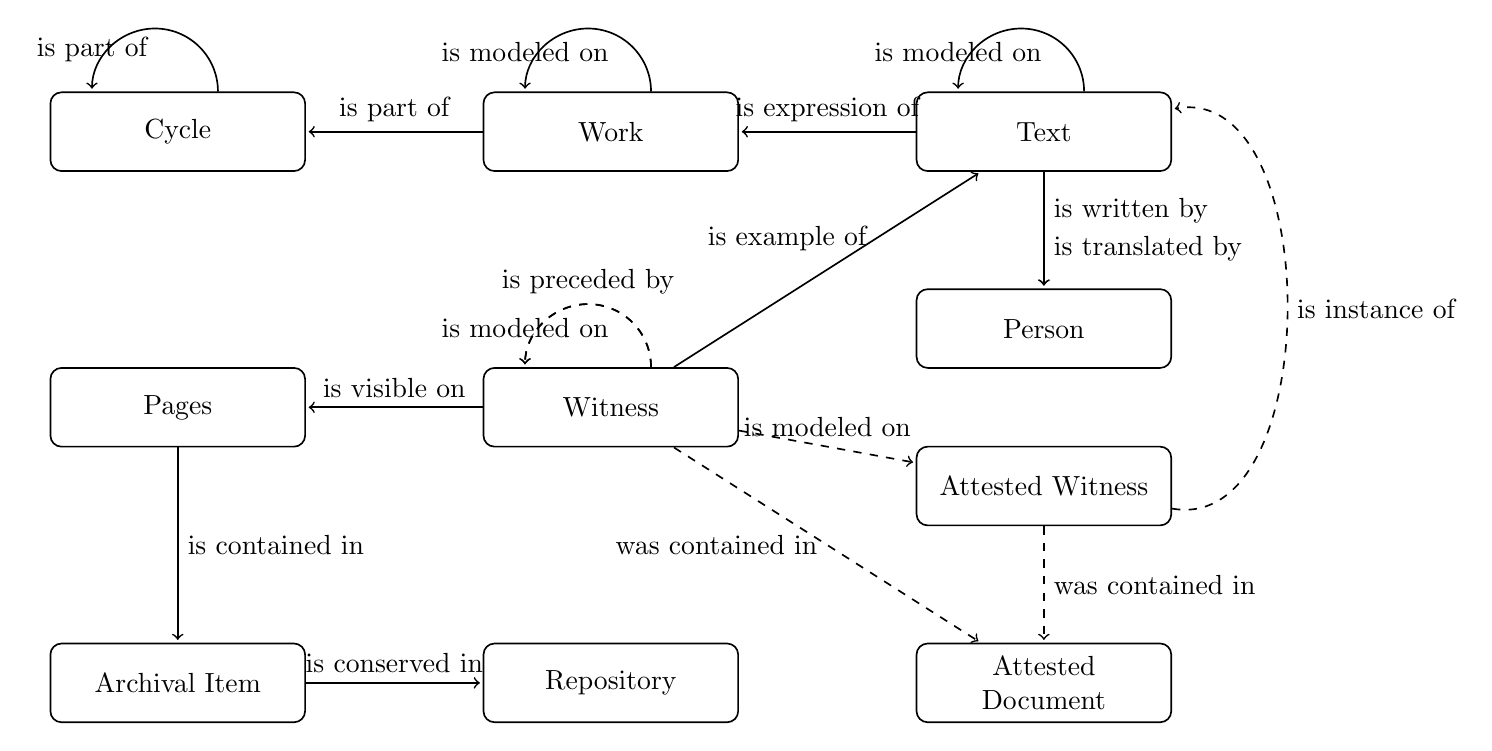
\begin{tikzpicture}[-,shorten >=1pt,auto,node distance=2.5cm,semithick]
\tikzstyle{every state}=[fill=red,draw=none,text=white]

\node[s] (cycle) [] {Cycle};
\node[s] (work) [right of=cycle, xshift=3cm] {Work};
\node[s] (text) [right of=work, xshift=3cm] {Text};

\node[s] (person) [below of=text] {Person};

\node[s] (attestedWitness) [below of=person, yshift=0.5cm] {Attested Witness};

\node[s] (witness) [below of=work, yshift=-1cm] {Witness};

\node[s] (pages) [left of=witness, xshift=-3cm] {Pages};

\node[s] (item) [below of=pages, yshift=-1cm] {Archival Item};

\node[s] (repo) [right of=item, xshift=3cm] {Repository};

\node[s] (document) [right of=repo, xshift=3cm] {Attested Document};

% \draw[dashed, ->] (witness.-45) arc (200:475:8mm) 
%   node[pos=0.5, below] () {is preceded by};
\draw[dashed, ->] (witness.45) arc (0:180:8mm)
  node[above, pos=0.5] () {is preceded by};
\draw[dashed, ->] (witness.45) arc (0:180:8mm)
  node[above, yshift=0.25cm] () {is modeled on};
\draw[->] (cycle.45) arc (0:180:8mm) 
  node[above, yshift=0.25cm] () {is part of};
\draw[->] (work.45) arc (0:180:8mm) 
  node[above, yshift=0.25cm] () {is modeled on};
\draw[->] (work) -- (cycle)
  node[pos=0.5, above] () {is part of};
\draw[->] (text) -- (work)
  node[pos=0.5, above] () {is expression of};
\draw[->] (witness) -- (text)
  node[pos=0.66, left] () {is example of};
\draw[dashed,->] (witness) -- (document)
  node[pos=0.5, left] () {was contained in};
\draw[->] (pages) -- (item)
  node[pos=0.5, right] () {is contained in};
\draw[->] (witness) -- (pages)
  node[pos=0.5, above] () {is visible on};
\draw[->] (item) -- (repo)
  node[pos=0.5, above] () {is conserved in};
\draw[->] (text.45) arc (0:180:8mm) 
  node[yshift=0.25cm, above] () {is modeled on};
\draw[->] (text) -- (person)
  node[pos=0.66, right] {is translated by};
\draw[->] (text) -- (person)
  node[pos=0.33, right] {is written by};
\draw[dashed, ->] (witness) -- (attestedWitness)
  node[pos=0.5, above] {is modeled on};
\draw[dashed, ->] (attestedWitness) -- (document)
  node[pos=0.5, right] {was contained in};

\path[every node]
  (attestedWitness) edge[dashed, ->, bend right=100] node [pos=0.5, right] {is instance of} (text)
  ;

\end{tikzpicture}
    \end{center}
\caption{Proposed Entities.}
\label{fig:ProposedEntities}
\end{figure}

\subsubsection{Archival Evidence}

Stemming from an extant \textit{Witness} are potentially four types of relationships to other entities. First and foremost, a \textit{Witness} must relate to one and only one \textit{Text}. By definition, a \textit{Witness} is an extant version of a \textit{Text's} linguistic content, spelled out in a sequence of characters, as demonstrated in Table \ref{tab:TextVersions}. Therefore, the \textit{Witness} must be the manifestation of a \textit{Text}. Second, the \textit{Witness}, by virtue of being extant, must be visible on the \textit{Pages} of an \textit{Archival Item}. When the version of a \textit{Text} has survived through fragments, one of the fragmented version's \textit{Witnesses} can relate to another fragment through the attribute ``is preceded by.'' An example of this inter-\textit{Witness} relationship is demonstrated in the case of the \textit{Chanson d'Aspremont} and the Table \ref{tab:CampsAspremont}. Finally, a \textit{Witness} can have formerly been contained in a document which has not survived but to whose historical existence scholars attest based on philological and codicological evidence.

\textit{Pages} represents an uninterrupted set of folios and, when digitized, images of an \textit{Archival Item} on which the text content of a \textit{Witness} can be read. In our data model, a \textit{Pages} entity, which depends on an extant \textit{Witness}, must be contained in an \textit{Archival Item}. The \textit{Archival Item} can relate to multiple \textit{Pages} entities. However, the first folio of one \textit{Pages} entity must not come before the last folio of another \textit{Pages} entity in the same \textit{Archival Item}. In other words, \textit{Pages} entities cannot overlap. They represent a unique set of leafs or pages in an \textit{Archival Item}, and they present the content of only one \textit{Witness}. Lastly, the \textit{Archival Item}, being an object one can consult and which continues to persist, contrary to the \textit{Attested Document}, must be conserved in a \textit{Repository}.

\subsubsection{Genealogy of a \textit{Text}}

While the proposed data model manages metadata about intertextuality within the corpus, its relational framework does not register how \textit{Witnesses} derive from one another. This choice reflects an assumption about intertextuality, meaning \textit{Works'} and \textit{Texts'} models, and stemma, meaning \textit{Witness'} models. On the one hand, we assume a relatively consistent consensus has been reached on the models of \textit{Works} and \textit{Texts}. We presume scholars and archivists have largely accepted as historical fact the assertion that one \textit{Text} is a translation of another \textit{Text}, that a \textit{Work} is a compilation of other \textit{Works}, that one \textit{Text} is the prose version of another \textit{Text}, and so on. Through analyses of the content and literary form of extant \textit{Witnesses} that are examples of \textit{Texts} and \textit{Works}, such claims of genealogy and intertextuality tend not to attract as much skepticism as claims about \textit{Witnesses} of a \textit{Text}. Scholars posit hypotheses that the scribes who arranged the spelling, phrasing, and formatting of one \textit{Witness} derived their version (Sahle's text-as-version) from another \textit{Witness}.

Such stemmatological claims are crucial, and we want to model them for the corpus. However, in addition to establishing a relationship between two \textit{Witness} entities, it is also critical to cite the source of that attested dependence. Furthermore, we want to permit conflicting stemma without over complicating the model's relationships. While it is possible to model such connections in a relational framework, exploiting those connections to respond to users' queries risks pushing the model to become over complex. The choice becomes one between exploting one over-complicated model or harmonizing and jointly exploiting two simpler models.

Rather than reinvent the wheel and model stemma in a complex relational framework, we propose pairing the former with a graph framework, which philologists have used for decades.\footcite[][]{Zundert2020} The relational framework's main tasks are, therefore, to generate entities relevant to our corpus, store metadata about them, and establish intertextual relations at the level of the abstract, narrative content, meaning the \textit{Work} and \textit{Text}. In conjunction, the graph database's \textit{Witness} nodes will bear the same identifier as their counterpart in the relational database and thus can be enriched with metadata.

The project \textit{OpenStemmata} has already designed a workflow through which contributors can encode stemma that have been published in a scholarly context or otherwise submitted by scholars. For example, Giovanni Palumbo and Paolo Rinoldi, who, while developing a critical edition of the French \textit{Chanson d'Aspremont}, produced a stemma of the first part of the \textit{Text}. Their stemma was encoded and uploaded to the \textit{OpenStemmata} database, and we have represented it here in Figure \ref{fig:GraphFramework}. The graph's gray node P\textsubscript{4} is equivalent to the \textit{Witness} P\textsubscript{4} in our earlier \textit{Chanson d'Aspremont} test case, as seen in Figures \ref{fig:BNFNAF5094}, \ref{fig:AspremontCFBNF}, and \ref{fig:WitnessRelations}.

\begin{figure}[ht]
    \begin{center}
        \tikzstyle{s} = [circle, minimum width=1cm, text width=1cm, minimum height=1cm, text centered, draw=black]
\tikzstyle{n} = [circle, minimum width=1cm, text width=1cm, minimum height=1cm, text centered, draw=black, fill=gray!30]
\tikzstyle{p} = [circle, minimum width=1cm, text width=1cm, minimum height=1cm, text centered, draw=black, line width=0.75mm, fill=gray!30]
\tikzstyle{arrow} = [thick,->,>=stealth]
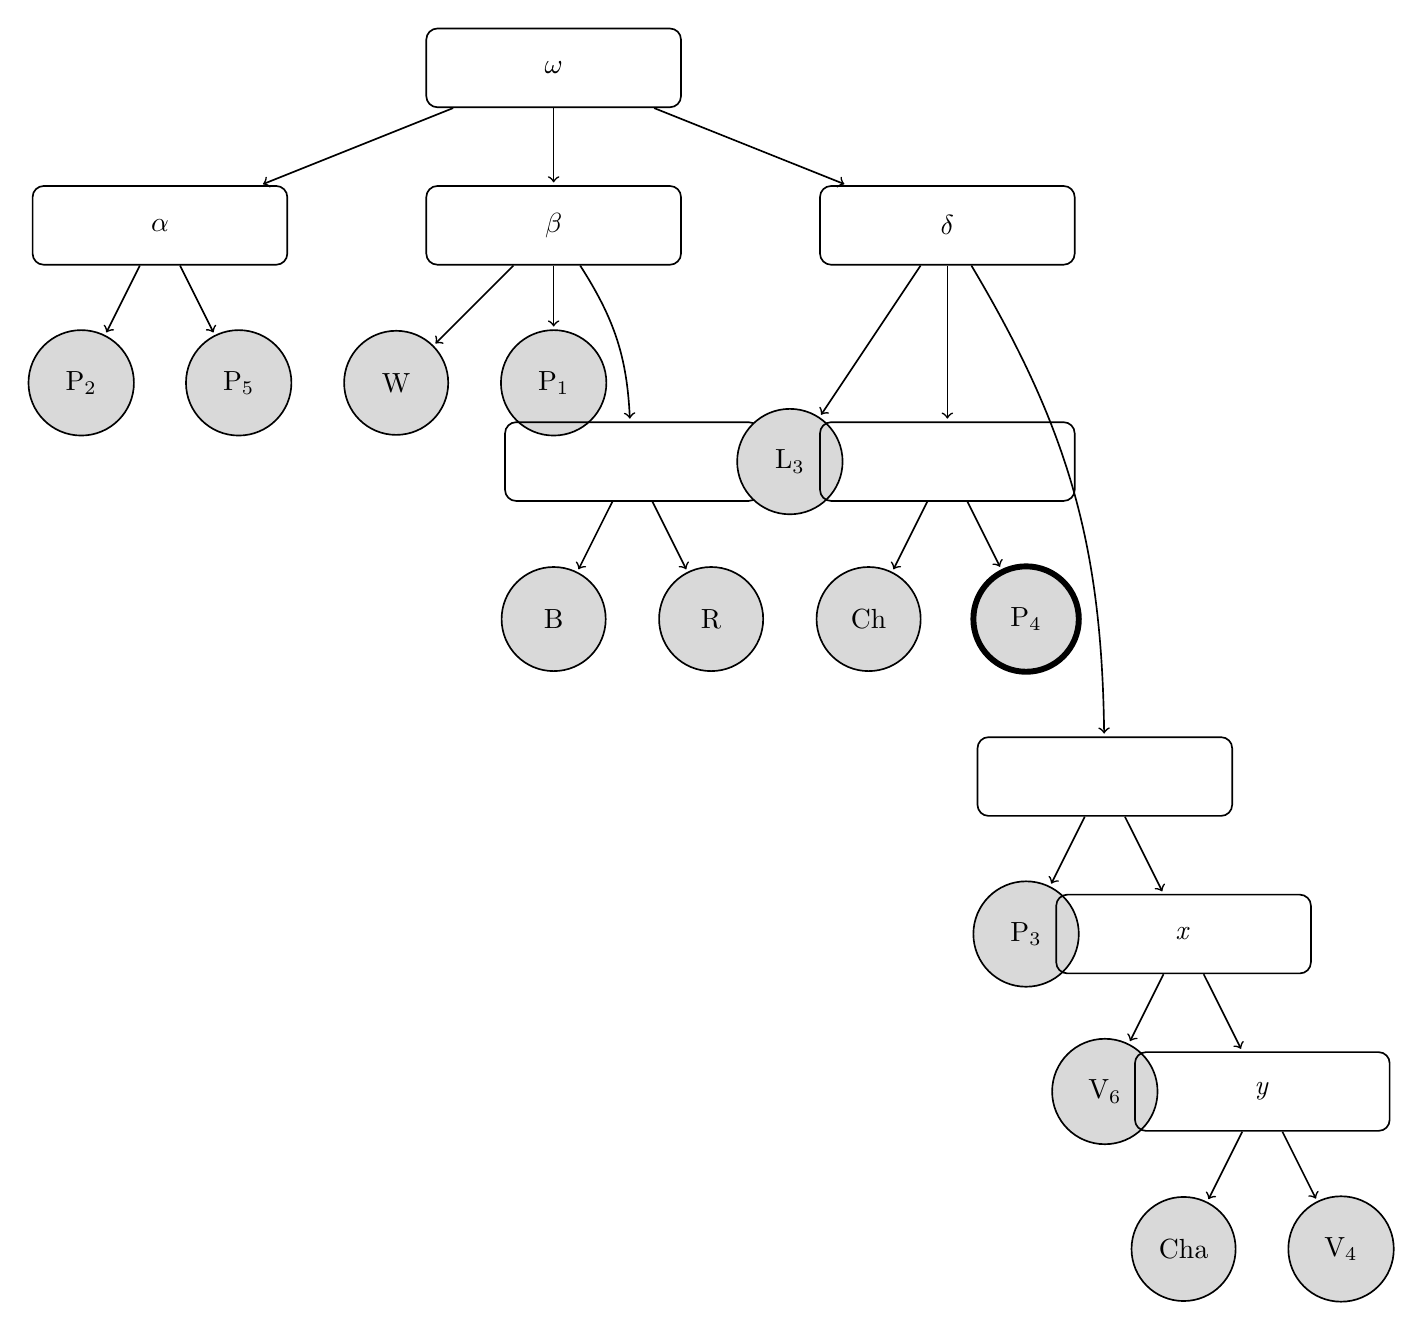
\begin{tikzpicture}[-,shorten >=1pt,auto,node distance=2cm,semithick]
\tikzstyle{every state}=[fill=red,draw=none,text=white]

\node[s] (w) {$\omega$};

\node[s] (a) [below of=w, xshift=-5cm] {$\alpha$};
\node[n] (p2) [below of=a, xshift=-1cm] {P\textsubscript{2}};
\node[n] (p5) [below of=a, xshift=1cm] {P\textsubscript{5}};

\path[every node/.style={font=\sffamily\small}]
    (w) edge[->] node[]{} (a)
    (a) edge[->] node[]{} (p2)
    (a) edge[->] node[]{} (p5)
;

\node[s] (b) [below of=w] {$\beta$};
\node[n] (W) [below of=b, xshift=-2cm] {W};
\node[n] (p1) [below of=b] {P\textsubscript{1}};
\node[s] (bb) [below of=b, yshift=-1cm, xshift=1cm] {};
\node[n] (B) [below of=bb, xshift=-1cm] {B};
\node[n] (R) [below of=bb, xshift=1cm] {R};

\path[every node/.style={font=\sffamily\small}]
    (w) edge[->] node[]{} (b)
    (b) edge[->] node[]{} (W)
    (b) edge[->] node[]{} (p1)
    (b) edge[->, bend left=15] node[]{} (bb)
    (bb) edge[->] node[]{} (B)
    (bb) edge[->] node[]{} (R)
;

\node[s] (d) [below of=w, xshift=5cm] {$\delta$};
\node[n] (l3) [below of=d, yshift=-1cm, xshift=-2cm] {L\textsubscript{3}};
\node[s] (dd1) [right of=l3] {};
\node[n] (ch) [below of=dd1, xshift=-1cm] {Ch};
\node[p] (p4) [below of=dd1, xshift=1cm] {P\textsubscript{4}};
\node[s] (dd2) [below of=d, xshift=2cm, yshift=-5cm] {};
\node[n] (p3) [below of=dd2, xshift=-1cm] {P\textsubscript{3}};
\node[s] (x) [below of=dd2, xshift=1cm] {\textit{x}};
\node[n] (v6) [below of=x, xshift=-1cm] {V\textsubscript{6}};
\node[s] (y) [below of=x, xshift=1cm] {\textit{y}};
\node[n] (cha) [below of=y, xshift=-1cm] {Cha};
\node[n] (v4) [below of=y, xshift=1cm] {V\textsubscript{4}};

\path[every node/.style={font=\sffamily\small}]
    (w) edge[->] node[]{} (d)
    (d) edge[->] node[]{} (l3)
    (d) edge[->] node[]{} (dd1)
    (dd1) edge[->] node[]{} (ch)
    (dd1) edge[->] node[]{} (p4)
    (d) edge[->, bend left=15] node[]{} (dd2)
    (dd2) edge[->] node[]{} (p3)
    (dd2) edge[->] node[]{} (x)
    (x) edge[->] node[]{} (v6)
    (x) edge[->] node[]{} (y)
    (y) edge[->] node[]{} (cha)
    (y) edge[->] node[]{} (v4)
;

\end{tikzpicture}

% \node[s] (w) {$\omega$};
% \node[s] (wl) [below of=w, xshift=-2cm] {};
% \node[s] (a) [below of=w, xshift=2cm] {$\alpha$};
% \node[s] (b) [below of=wl, xshift=-4cm] {$\beta$};
% \node[s] (gamma) [below of=wl] {$\gamma$};
% \node[n] (W) [below of=b, xshift=-2cm] {W};
% \node[n] (p5) [below of=b] {P\textsubscript{5}};
% \node[s] (gammal) [below of=gamma] {};
% \node[n] (l3) [below of=gammal, xshift=-2cm] {L\textsubscript{3}};
% \node[n] (ch) [below of=gammal] {Ch};
% \node[s] (x) [below of=gamma, xshift=2cm] {\textit{x}};
% \node[s] (y) [below of=x] {\textit{x}};
% \node[n] (cha) [below of=y, xshift=-1cm] {Cha};
% \node[n] (v4) [below of=y, xshift=1cm] {V\textsubscript{4}};
% \node[n] (v6) [below of=x, xshift=2cm] {V\textsubscript{6}};
% \node[n] (p2) [below of=a] {P\textsubscript{2}};
% \node[n] (p3) [below of=a, xshift=2cm] {P\textsubscript{3}};
% \node[n] (l2) [below of=a, xshift=4cm] {L\textsubscript{2}};

% \path[every node/.style={font=\sffamily\small}]
%     (w) edge[->] node[]{} (a)
%     (w) edge[->] node[]{} (wl)
%     (wl) edge[->] node[]{} (b)
%     (wl) edge[->] node[]{} (gamma)
%     (b) edge[->] node[]{} (W)
%     (b) edge[->] node[]{} (p5)
%     (gamma) edge[->] node[]{} (gammal)
%     (gamma) edge[->] node[]{} (x)
%     (gammal) edge[->] node[]{} (l3)
%     (gammal) edge[->] node[]{} (ch)
%     (x) edge[->] node[]{} (y)
%     (x) edge[->] node[]{} (v6)
%     (y) edge[->] node[]{} (cha)
%     (y) edge[->] node[]{} (v4)
%     (a) edge[->] node[]{} (p2)
%     (a) edge[->] node[]{} (p3)
%     (a) edge[->] node[]{} (l2)
% ;

% \end{tikzpicture}
    \end{center}
\caption{Stemma of extant \textit{Witnesses} (gray) and supposed witnesses (white) of the first part of the French \textit{Chanson d'Aspremont} by G. Palumbo and P. Rinoldi.}
\label{fig:GraphFramework}
\end{figure}

We propose outsourcing the data model's \textit{Text} genealogies to the \textit{OpenStemmata} project's established workflow, encoding standards, and open-source repository. Subsequently, we reconcile the \textit{Witness} nodes in the \textit{OpenStemmata} database, further valorizing and enriching those publications, with records registered in our proposed relational data model. Finally, having linked the two record types, such as the \textit{Witness} P\textsubscript{4} of the Anglo-Norman \textit{Chanson d'Aspremont}, the data model can deliver thoroughly enriched and linked records based on users' requests.

\subsubsection{Reconciling and citing records}

Finally, we propose a \textit{Reference} table, which associates certain entities with bibliographic resources. This last addition serves two purposes. First, it associates an entity with a unique identifier in an authoritative aggregator, such as WikiData, Biblissima, and VIAF (Virtual International Authority File). This association helps reconcile potentially duplicate records in the data model and helps reconcile records between the relational data model and an \textit{OpenStemmata} graph. Second, \textit{Reference} associates entities with scholarly citations. In addition to making the data model interoperable with other databases, including VIAF, the \textit{Reference} entity also allows us to enrich records with a scholarly bibliography.

\begin{figure}[ht]
    \begin{center}
        \input{sections/figures/proposed-entities-reference.tex}
    \end{center}
\caption{Proposed Entities with \textit{Reference} table.}
\label{fig:ProposedEntitiesReference}
\end{figure}

\textit{Reference} can reconcile conflicting \textit{Cycle}, \textit{Work}, \textit{Text}, \textit{Person}, and \textit{Archival Item} entities and link them to universal unique identifiers. The \textit{Archival Item} entity should ideally have an Archival Resource Key provided by its \textit{Repository}, which should help avoid duplicate records of the same manuscript. The entities \textit{Cycle}, \textit{Work}, and \textit{Person} have overlap with entities in the VIAF database; our model's \textit{Person} is equivalent to VIAF's \textit{Personal Names} and our model's \textit{Cycle}, \textit{Work}, \textit{Text} records can find equivalent under VIAF's \textit{Work} and \textit{Expression} records. The latter two entities in the VIAF model are borrowed from the FRBR.

For example, the \textit{Work} \textit{Renaut de Montauban}, seen in Table \ref{sub:Work}, has the VIAF identifier {\texttt{174185484}}, as seen in the last row of Table \ref{sub:Reference}. By linking a \textit{Work} record to a \textit{Reference} record, which in this case associates \textit{Renaut de Montauban} with an identifier in the VIAF database, we can enrich the \textit{Work} with all the linked data available in VIAF. Furthermore, while our record for \textit{Renaut de Montauban} has one title, its link to the VIAF database via the \textit{Reference} entity associates the \textit{Work} with other names by which people might identify it, including \textit{Renaud de Montauban}, \textit{Reinolt von Montelban}, and \textit{Quatre fils Aymon}, further improving the data's interoperability and resilience against duplication.

\begin{figure}[ht]

    \begin{subfigure}{\textwidth}
        \begin{center}
        \begin{tabular}{|p{0.05\textwidth}|p{0.2\textwidth}|p{0.1\textwidth}|}
            \hline
            \textbf{ID} & \textbf{title} & \textbf{is part of} \\ \hline
            1 & Renaut de Montauban & \\ \hline
        \end{tabular}
        \end{center}
    \subcaption{\textit{Cycle} record for \textit{Renaut de Montauban}.}
    \label{sub:Cycle}
    \vspace*{1em}
    \end{subfigure}

    \begin{subfigure}{\textwidth}
        \begin{center}
        \begin{tabular}{|p{0.05\textwidth}|p{0.2\textwidth}|p{0.1\textwidth}|p{0.15\textwidth}|}
            \hline
            \textbf{ID} & \textbf{title} & \textbf{is part of} & \textbf{is modeled on} \\ \hline
            2 & Renaut de Montauban & 1 & \\ \hline
        \end{tabular}
        \end{center}
    \subcaption{\textit{Work} record for \textit{Renaut de Montauban}.}
    \label{sub:Work}
    \vspace*{1em}
    \end{subfigure}

    \begin{subfigure}{\textwidth}
        \begin{center}
        \begin{tabular}{|p{0.05\textwidth}|p{0.05\textwidth}|p{0.1\textwidth}|p{0.1\textwidth}|p{0.2\textwidth}|p{0.3\textwidth}|}
            \hline
            \textbf{entity type} & \textbf{entity ID} & \textbf{unique identifier} & \textbf{identifier source} & \textbf{permalink} & \textbf{citation} \\ \hline
            Cycle & 1 & & & & \cite{Augustine2020} \\ \hline
            Cycle & 1 & 5045 & Arlima & \url{https://arlima.net/no/5045} & \\ \hline
            Cycle & 1 & Q59212800 & WikiData & \url{https://www.wikidata.org/wiki/Q59212800} & \\ \hline
            Work & 2 & 318 & Arlima & \url{https://arlima.net/no/318} & \\ \hline
            Work & 2 & Q115962675 & WikiData & \url{https://www.wikidata.org/wiki/Q115962675} & \\ \hline
            Work & 2 & 174185484 & VIAF & \url{http://viaf.org/viaf/174185484} & \\ \hline
        \end{tabular}
        \end{center}
    \subcaption{\textit{Reference} records for \textit{Renaut de Montauban}.}
    \vspace*{1em}
    \label{sub:Reference}
    \end{subfigure}

\label{tab:ReferenceRenaut}
\end{figure}

%%%%%%%%%%%%%%%%%%%%%%%%%

\subsection{Cycle}

Definition: General theme that a group of \textit{Works} can share.  

\vspace{1em}
\noindent Attributes:
\begin{itemize}
    \item \texttt{title} (text, req., uniq.): Received name of the \textit{Cycle}, either in the language of the first known \textit{Text} to treat the matter or in the language most used in scholarship.
    \item \texttt{is part of} (foreign key, \textbf{Cycle}, opt., uniq.): The meta-\textit{Cycle}, of which the \textit{Cycle} is a part.
\end{itemize}

\begin{figure}[ht]
    \begin{center}
        \tikzstyle{s} = [rectangle, rounded corners, minimum width=2cm, text width=3cm, minimum height=1cm, text centered, draw=black]
\tikzstyle{arrow} = [thick,->,>=stealth]
\begin{tikzpicture}[-,shorten >=1pt,auto,node distance=1.5cm,semithick]
\tikzstyle{every state}=[fill=red,draw=none,text=white]

\pic [] { entityassociative = {{cycle}
{\textbf{Cycle}}
{
  \textbf{ID} \\
  \hline
  title \\
  is part of \\
}
}};

\pic [right = 15em of cycle] { entityassociative = {{work}
{\textbf{Work}}
{
  \textbf{ID} \\
  \hline
  title \\
  is part of \\
}
}};


\draw[one-many] (cycle.east) -- node[label, above]{Cycle has 1 or more} (work.west);
\draw[one-many] (cycle.east) -- node[label, below]{Works that are part of it}(work.west);

\end{tikzpicture}
    \end{center}
\label{fig:CycleER}
\caption{\textit{Cycle} entity relationships.}
\end{figure}

%%%%%%%%%%%%%%%%%%%%%%%%%

\subsection{Work}

Definition: Content of a story, which has a recognizable structure and can be recounted in different ways while remaining the same story.

\vspace{1em}
\noindent Attributes:
\begin{itemize}
    \item \texttt{title} (text, req., uniq.): Received name of the \textit{Work}, either in the language of the first known \textit{Text} to treat the matter or in the language most used in scholarship.
    \item \texttt{is part of} (foreign key, \textbf{Cycle}, opt., uniq.): The \textit{Cycle}, of which the \textit{Work} is a part.
    \item \texttt{is modeled on} (foreign key, \textbf{Work}, opt., repeat.): If a reworking of an anterior \textit{Work}, the \textit{Work} on which it is modeled.
\end{itemize}


\begin{figure}[ht]
    \begin{center}
        \tikzstyle{s} = [rectangle, rounded corners, minimum width=2cm, text width=3cm, minimum height=1cm, text centered, draw=black]
\tikzstyle{arrow} = [thick,->,>=stealth]
\begin{tikzpicture}[-,shorten >=1pt,auto,node distance=1.5cm,semithick]
\tikzstyle{every state}=[fill=red,draw=none,text=white]

\pic [] { entityassociative = {{cycle}
{\textbf{Cycle}}
{
  \textbf{ID} \\
  \hline
  title \\
  is part of \\
}
}};

\pic [right = 12em of cycle] { entityassociative = {{work}
{\textbf{Work}}
{
  \textbf{ID} \\
  \hline
  title \\
  is part of \\
  is modeled on \\
}
}};


\pic [right = 12em of work] { entityassociative = {{text}
{\textbf{Text}}
{
  \textbf{ID} \\
  \hline
  is expression of \\
  is modeled on \\
  title \\
  person creator \\
  person translator \\
  creation date \\
  creation date text \\
  creation date cite \\
  matter \\
  regional genre\\
  language\\
  form\\
  poetic meter\\
  rhyme type \\
  strophe count \\
  strophe length \\
  verse length \\
}
}};

\pic [below = 5em of work] { entityassociative = {{reference}
{\textbf{Reference}}
{
  entity type\\
  entity ID \\
  unique identifier \\
  identifier source \\
  citation \\
}
}};

\draw[omany-omany] (reference) -- node[label, left, pos=0.5]{Work has 0, 1, or many References} (work);

\draw[one-omany] (cycle.east) -- node[label, above]{Work is part of} (work.west);
\draw[one-omany] (cycle.east) -- node[label, below]{1 and only 1 Cycle} (work.west);

\draw[one-many] (work.east) -- node[label, above]{Work has 1 or more} (text.west);
\draw[one-many] (work.east) -- node[label, below]{Text expressions} (text.west);

\end{tikzpicture}
    \end{center}
\label{fig:WorkER}
\caption{\textit{Work} entity relationships.}
\end{figure}

%%%%%%%%%%%%%%%%%%%%%%%%%

\subsection{Text}

Definition: Formulation of a \textit{Work} in human language, whose literary form and style can be detected and whose creation can be attributed to one or more individuals.

\vspace{1em}
\noindent Attributes:
\begin{itemize}
    \item \texttt{is expression of} (foreign key [\textbf{Work}], req., uniq.): The \textit{Work} that the \textit{Text} articulates.
    \item \texttt{is modeled on} (foreign key, [\textbf{Text}], opt., uniq.): If the \textit{Text} is derived from another \textit{Text}, a reference to the model \textit{Text}.
    \item \texttt{title} (text, req., uniq.): Either the given title of the \textit{Text}, as provided by the creator, or the standardized title most used in scholarship to refer to the \textit{Text}.
    \item \texttt{is written by} (foreign key [\textbf{Person}], opt., repeat.): The individual accredited with composing the \textit{Text}.
    \item \texttt{is translated by} (foreign key [\textbf{Person}], opt., repeat.): When the \textit{Text} is a translation of another \textit{Text}, the individual accredited with creating the translation.
    \item \texttt{creation date} (list[date], opt., uniq.): A list of two or one dates; the first date is either the earliest or the only date associated with the \textit{Text's} creation, and, in the case of a range, the second date is the latest date associated with the creation.
    \item \texttt{creation date text} (text, opt., uniq.): The date associated with the \textit{Text's} creation as it is written in a scholarly source.
    \item \texttt{creation date cite} (text, opt., uniq.): A citation of the source that provided the date of creation.
    \item \texttt{matter} (terms, opt., repeat.): The matter treated in the \textit{Text}, as defined by Jean Bodel.
    \begin{itemize}
        \item \texttt{Britain}: Matter of Britain, which includes stories about Tristan and King Arthur.
        \item \texttt{France}: Matter of France, which includes stories about Charlemagne.
        \item \texttt{Rome}: Matter of Rome, which includes stories about Troy, Rome, Alexander, and antiquity.
    \end{itemize}
    \item \texttt{regional genre} (terms, req., uniq.): Literary genre attributed to the \textit{Text}.
    \begin{multicols}{2}
        \begin{itemize}
            \item Relevant to French tradition
                \begin{itemize}
                    \item \texttt{chanson de geste}: i.e. \textit{Girartz de Rossilho}
                    \item \texttt{roman}
                \end{itemize}
            \item Relevant to Iberian tradition
            \begin{itemize}
                \item \texttt{romancero}: i.e. \textit{Cantar de mio Cid}
                \item \texttt{novela}: 
            \end{itemize}
            \item Relevant to Italian tradition
            \begin{itemize}
                \item \href{https://www.oxfordbibliographies.com/display/document/obo-9780195396584/obo-9780195396584-0199.xml}{\texttt{cantare}}
                \item \texttt{poema cavalleresche}
            \end{itemize}
            \item Relevant to Islandic tradition
                \begin{itemize}
                    \item \texttt{fornaldarsögur}
                    \item \texttt{riddarasögur}
                    \item \texttt{rímur}
                    \item \texttt{fornaldarrímur}
                    \item \texttt{riddararímur}
                \end{itemize}
            \item Relevant to Middle Dutch tradition
                \begin{itemize}
                    \item \texttt{ridderepiek}: i.e. \textit{Roman van Moriaen}
                    \item \texttt{ridderroman}: i.e. \textit{Arthurs doet}
                    \item \texttt{rijmkronieken}: i.e. \textit{Brabantsche Yeesten}
                \end{itemize}
            \item Relevant to Middle English, Middle Irish, Middle Welsh traditions
            \begin{itemize}
                \item \texttt{romance}
            \end{itemize}
            \item Relevant to Middle High German tradition
        \end{itemize}
    \end{multicols}
    \item \texttt{language} (terms, req., uniq.): ISO code of the primary language through which the \textit{Text} expresses the \textit{Work}.
    \begin{multicols}{2}
        \begin{itemize}
            \item \texttt{cat}: Catalan
            \item \texttt{dum}: Middle Dutch
            \item \texttt{enm}: Middle English (1100-1500)
            \item \texttt{frm}: Middle French (ca. 1400-1600)
            \item \texttt{fro}: Old French (842-ca. 1400)
            \item \href{https://www.wikidata.org/wiki/Q54879035}{\texttt{fro\_ITA}}: Franco-Italian
            \item \texttt{fro\_PRO}: Franco-Occitan
            \item \texttt{ghg}: Hiberno-Scottish Gaelic, Early Modern Irish
            \item \texttt{glg}: Galician
            \item \href{https://www.wikidata.org/wiki/Q1072111}{\texttt{glg\_POR}}: Galician-Portugese
            \item \texttt{gmh}: Middle High German (ca. 1050-1500)
            \item \texttt{gml}: Middle Low German
            \item \texttt{isl}: Islandic
            \item \texttt{ita}: Italian
            \item \texttt{mga}: Middle Irish (900-1200)
            \item \texttt{non}: Old Norse
            \item \href{https://www.wikidata.org/wiki/Q12330003}{\texttt{non\_DAN}}: Old East Norse, Old Danish (800-1100)
            \item \href{https://www.wikidata.org/wiki/Q2417210}{\texttt{non\_SWE}}: Old Swedish (800-1500)
            \item \texttt{oco}: Old Cornish
            \item \texttt{por}: Portugese
            \item \texttt{pro}: Old Occitan, Old Provençal (to 1500)
            \item \texttt{spa}: Spanish or Castilian
            \item \texttt{wlm}: Middle Welsh
            \item \href{https://data.biblissima.fr/w/Item:Q286307}{\texttt{xno}}: Anglo-French, Anglo-Norman
        \end{itemize}
    \end{multicols}
    \item \texttt{form} (terms, req., uniq.): Whether the \textit{Text} is formed in prose, verse, or a mix of both.
    \begin{multicols}{4}
        \begin{itemize}
            \item \texttt{prose}
            \item \texttt{verse}
            \item \texttt{mixed}
        \end{itemize}
    \end{multicols}
    \item \texttt{poetic meter} (terms, opt., uniq.): If the \textit{Text} is in verse, the type of poetic meter.
        \begin{itemize}
            \item \texttt{French alexandrine}: line consisting of 2 half-lines each of 6 syllables, total of 12 syllables.
            \item \texttt{dodecasyllabe}: line consisting of 12 syllables.
            \item \texttt{decasyllabe}: line consisting of 10 syllables.
            \item \texttt{octosyllabe}: line consisting of 8 syllables.
            \item \texttt{hexasyllabe}: line consisting of 6 syllables.
            \item \texttt{pentasyllabe}: line consisting of 5 syllables.
        \end{itemize}
    \item \texttt{rhyme type} (terms, opt., repeat.): If the \textit{Text} is in verse, the types of rhyme used.
        \begin{itemize}
            \item \texttt{alliteration}: Rhyme is allowed between words that either start with the same consonant sound or with the same vowel, such as ``\textit{With floures fele, fair under fete}'' in Middle English.\footcite[][396]{Davis2002}
            \item \texttt{assonance}: Rhyme is allowed between words that have a repeated vowel sound, such as ``a'' in ``\textit{Vio puertas abiertas e uços sin cañados / alcandaras vazias sin pielles e sin mantos}'' in Castilian.\footcite[][364]{Gornall1995}
            \item \texttt{end-rhyme}: Rhyme is allowed between words that have an ending that sounds the same, such as ``\textit{ihesu guz son ihesu goþe / bløt mit hiærta mæþ þino bloþe}'' in Old Norse.\footcite[][423]{Layher2008}
            \item \texttt{generic}: ``[R]hyme is allowed between any one member of a phonetic group and is itself or any other member of the same group,'' such as `b,' `g,' `d' in Old Irish.\footcite[][822]{McKie1997}
        \end{itemize}
    \item \texttt{strophe count} (integer, opt., uniq.): If the \textit{Text} is in verse and strophic, the number of strophes.
    \item \texttt{strophe length} (integer, opt., uniq.): If the \textit{Text} is in verse and strophic, the number of lines in each strophe.
    \item \texttt{verse length} (integer, opt., uniq.): If the \textit{Text} is in verse, the number of verses a complete version (\textit{Witness}) of it should have.
\end{itemize}

\begin{figure}[ht]
    \begin{center}
        \tikzstyle{s} = [rectangle, rounded corners, minimum width=2cm, text width=3cm, minimum height=1cm, text centered, draw=black]
\tikzstyle{arrow} = [thick,->,>=stealth]
\begin{tikzpicture}[-,shorten >=1pt,auto,node distance=1.5cm,semithick]
\tikzstyle{every state}=[fill=red,draw=none,text=white]

\pic [] { entityassociative = {{text}
{\textbf{Text}}
{
  \textbf{ID} \\
  \hline
  is expression of \\
  is modeled on \\
  title \\
  is written by \\
  is translated by \\
  creation date \\
  creation date text \\
  creation date cite \\
  matter \\
  regional genre\\
  language\\
  form\\
  poetic meter\\
  rhyme type \\
  strophe count \\
  strophe length \\
  verse length \\
}
}};

\pic [left = 12em of text] { entityassociative = {{work}
{\textbf{Work}}
{
  \textbf{ID} \\
  \hline
  title \\
  is part of \\
}
}};

\pic [right = 12em of text] { entityassociative = {{witness}
{\textbf{Witness}}
{
  \textbf{ID} \\
  \hline
  is manifestation of\\
  is preceded by fragm.\\
  is preceded by wit.\\
  is visible on\\
  was contained in\\
  siglum \\
  status \\
  TEI document\\
  IIIF manifest\\
  scribe\\
  scripta\\
  creation date\\
  creation date text\\
  note\\
}
}};

\pic [below = 7em of text] { entityassociative = {{person}
{\textbf{Person}}
{
  \textbf{ID} \\
  \hline
  name \\
  note
}
}};

\pic [above = 7em of text] { entityassociative = {{reference}
{\textbf{Reference}}
{
  entity type\\
  entity ID \\
  unique identifier \\
  identifier source \\
  permalink\\
  citation \\
}
}};

\draw[omany-omany] (reference) -- node[label, pos=0.5, right]{Text has 0, 1, or many References} (text);

\draw[one-omany] (text) -- node[label, above, yshift=0.10cm]{Text is manifest in 0, 1, or} (witness);
\draw[one-omany] (text) -- node[label, below, yshift=-0.10cm]{many Witnesses} (witness);

\draw[one-many] (text) -- node[label, above, yshift=0.10cm]{Text is expression of} (work);
\draw[one-many] (text) -- node[label, below, yshift=-0.10cm]{1 and only 1 Work} (work);

\draw[omany-omany] (text) -- node[label, pos=0.40, right]{Text is written by 0, 1, or many Persons} (person);
\draw[omany-omany] (text) -- node[label, pos=0.60, right]{Text is translated by 0, 1, or many Persons} (person);

\end{tikzpicture}
    \end{center}
\label{fig:TextER}
\caption{\textit{Text} entity relationships.}
\end{figure}

%%%%%%%%%%%%%%%%%%%%%%%%%

\subsection{Person}

Definition: An individual bearing some responsibility for a \textit{Text} in the data set, either as a creator/author or as a translator, in the case of a \textit{Text} that is the translation of a model \textit{Text} in another language.

\vspace{1em}
\noindent Attributes:
\begin{itemize}
    \item \texttt{name} (text, req., uniq.): The recieved name of the individual.
    \item \texttt{note} (text, opt., uniq.): Optional notes to help identify the individual.
\end{itemize}

\begin{figure}[ht]
    \begin{center}
        \tikzstyle{s} = [rectangle, rounded corners, minimum width=2cm, text width=3cm, minimum height=1cm, text centered, draw=black]
\tikzstyle{arrow} = [thick,->,>=stealth]
\begin{tikzpicture}[-,shorten >=1pt,auto,node distance=1.5cm,semithick]
\tikzstyle{every state}=[fill=red,draw=none,text=white]

\pic [] { entityassociative = {{text}
{\textbf{Text}}
{
  \textbf{ID} \\
  \hline
  is expression of \\
  is modeled on \\
  title \\
  is written by \\
  is translated by \\
  creation date \\
  creation date text \\
  creation date cite \\
  matter \\
  regional genre\\
  language\\
  form\\
  poetic meter\\
  rhyme type \\
  strophe count \\
  strophe length \\
  verse length \\
}
}};


\pic [right = 10em of text] { entityassociative = {{person}
{\textbf{Person}}
{
  \textbf{ID} \\
  \hline
  name \\
  note
}
}};

\pic [right = 10em of person] { entityassociative = {{reference}
{\textbf{Reference}}
{
  entity type\\
  entity ID \\
  unique identifier \\
  identifier source \\
  permalink\\
  citation \\
}
}};

\draw[omany-omany] (reference) -- node[label, above, pos=0.5]{Person has 0, 1, or} (person);
\draw[omany-omany] (reference) -- node[label, below, pos=0.5]{many References} (person);

\draw[omany-omany] (text) -- node[label, above]{Person wrote/translated} (person);
\draw[omany-omany] (text) -- node[label, below]{0, 1, or many Texts} (person);

\end{tikzpicture}
    \end{center}
\label{fig:PersonER}
\caption{\textit{Person} entity relationships.}
\end{figure}

%%%%%%%%%%%%%%%%%%%%%%%%%

\subsection{Witness}

Definition: An extant manifestation of a \textit{Text} in a defined sequence of characters, which have been inscribed on a physical document.

\vspace{1em}
\noindent Attributes:
\begin{itemize}
    \item \texttt{is manifestation of} (foreign key [\textbf{Text}], req., uniq.): The \textit{Text} whose linguistic content the \textit{Witness} manifests in writing.
    \item \texttt{is preceded by} (foreign key [\textbf{Witness}], opt., uniq.): If the \textit{Witness} is a fragment, reference to another \textit{Witness} fragment, with which the \textit{Witness} is thought to have been produced in an original document, and which presents an earlier part of the \textit{Text} than its own part.
    \item \texttt{is visible on} (foreign key [\textbf{Pages}], opt., repeat.): 
    \item \texttt{was contained in} (foreign key [\textbf{Attested Document}], opt., uniq.): 
    \item \texttt{siglum} (text, opt., repeat.): Identifier used by scholars to indicate the extant \textit{Witness} within the \textit{Text's} tradition.
    \item \texttt{status} (terms, req., uniq.): Status of the extant \textit{Witness}.
    \begin{itemize}
        \item \texttt{complete}: All pages containing the main textual content of the \textit{Witness}, excluding dedications and decorations, have survived.
        \item \texttt{mutilated}: The \textit{Witness} presents parts of its \textit{Text} on a set of surviving pages ($ \geq 3 $ pages).
        \item \texttt{fragment}: Only a few pages of the \textit{Witness} survive ($ \leq 2 $ pages). 
        \item \texttt{citation}: The \textit{Witness} testifies to the existence of a \textit{Text}, through citation, but does not present all of the latter's linguistic content.
    \end{itemize}
    \item \texttt{TEI document} (text, opt., uniq.): Reference to a TEI-XML file representing the text content of the \textit{Witness}.
    \item \texttt{IIIF manifest} (text, opt., uniq.): Reference to a IIIF manifest JSON file representing the digitized images of the \textit{Witness's} \textit{Pages}.
    \item \texttt{scribe} (text, opt., uniq.): When known, identifying information about the scribe alleged to have written the text version.
    \item \texttt{scripta} (terms, opt., uniq.): When known, the name of a regional writing style, similar to the written version of a spoken dialect, as defined by Louis Remacle.\footcite[``Je désigne la langue vulgaire écrite au moyen âge par le néologisme \textit{scripta}. L'expression `la scripta' est synonyme de l'allemand `die Schriftsprache.'''][24]{Remacle1948}
    \item \texttt{creation date} (list[date], opt., uniq.): A list of two or one dates; the first date is either the earliest or the only date associated with the \textit{Witness's} production, and, in the case of a range, the second date is the latest date associated with the production.
    \item \texttt{creation date text} (text, opt., uniq.): The date associated with the \textit{Witness's} production as it is written in a catalogue or other scholarly source.
    \item \texttt{note} (text, opt., uniq.): Notes about the \textit{Witness} that will not be standardized and used in computational methods but may serve to protect the integrity of the record.
\end{itemize}

\begin{figure}[ht]
    \begin{center}
        \tikzstyle{s} = [rectangle, rounded corners, minimum width=2cm, text width=3cm, minimum height=1cm, text centered, draw=black]
\tikzstyle{arrow} = [thick,->,>=stealth]
\begin{tikzpicture}[-,shorten >=1pt,auto,node distance=1.5cm,semithick]
\tikzstyle{every state}=[fill=red,draw=none,text=white]

\pic [] { entityassociative = {{witness}
{\textbf{Witness}}
{
  \textbf{ID} \\
  \hline
  \textbf{Text ID} \\
  siglum \\
  status \\
  TEI document\\
  scribe\\
  scripta\\
  creation date\\
  is preceded by\\
  was contained in
}
}};

\pic [left = 12em of witness] { entityassociative = {{text}
{\textbf{Text}}
{
  \textbf{ID} \\
  \hline
  is expression of \\
  is modeled on \\
  title \\
  person creator \\
  person translator \\
  creation date \\
  creation date text \\
  creation date cite \\
  matter \\
  regional genre\\
  language\\
  form\\
  poetic meter\\
  stanza length \\
  verse length \\
  rhyme perfection\\
}
}};

\pic [right = 12em of witness] { entityassociative = {{pages}
{\textbf{Pages}}
  {
    \textbf{ID} \\
    \hline
    title \\
    is example of \\
    siglum \\
    siglum source \\
    status \\
    scribe \\
    scripta \\
  }
}};

\draw[one-omany] (text) -- node[label,above]{Witness is instance} (witness);
\draw[one-omany] (text) -- node[label,below]{of 1 and only 1 Text} (witness);

\draw[one-omany] (witness) --node[label, above]{Witness is visible} (pages);
\draw[one-omany] (witness) --node[label, below]{on 0 or many Pages} (pages);



\end{tikzpicture}
    \end{center}
\label{fig:WitnessER}
\caption{\textit{Witness} entity relationships.}
\end{figure}

%%%%%%%%%%%%%%%%%%%%%%%%%

\subsection{Pages}

Definition: An uninterrupted series of leafs or pages in an \textit{Archival Item} on which is inscribed the \textit{Witness} of a \textit{Text}.

\vspace{1em}
\noindent Attributes:
\begin{itemize}
    \item \texttt{is contained in}
    \item \texttt{archival item part}
    \item \texttt{witness part no}
    \item \texttt{folio start}
    \item \texttt{folio end}
    \item \texttt{image start}
    \item \texttt{image end}
\end{itemize}

\begin{figure}[ht]
    \begin{center}
        \tikzstyle{s} = [rectangle, rounded corners, minimum width=2cm, text width=3cm, minimum height=1cm, text centered, draw=black]
\tikzstyle{arrow} = [thick,->,>=stealth]
\begin{tikzpicture}[-,shorten >=1pt,auto,node distance=1.5cm,semithick]
\tikzstyle{every state}=[fill=red,draw=none,text=white]

\pic [] { entityassociative = {{pages}
{\textbf{Pages}}
{
    \textbf{ID} \\ \hline
    is contained in \\
    archival item part \\
    witness part \\
    folio start \\
    folio end \\
    image start \\
    image end \\
}
}};

\pic [left = 12em of pages] { entityassociative = {{witness}
{\textbf{Witness}}
{
  \textbf{ID} \\
  \hline
  is manifestation of\\
  is preceded by\\
  is visible on\\
  was contained in\\
  siglum \\
  status \\
  TEI document\\
  IIIF manifest\\
  scribe\\
  scripta\\
  creation date\\
  creation date text\\
  note\\
}
}};

\pic [right = 12em of pages] { entityassociative = {{item}
{\textbf{Archival Item}}
{
  \textbf{ID} \\
  \hline
  is conserved in\\
  collection\\
  shelfmark\\
  belatedly compiled\\
  provenance\\
  digitisation URL\\
  IIIF manifest\\
}
}};

\draw[one-omany] (witness) --node[label, above]{Pages makes visible} (pages);
\draw[one-omany] (witness) --node[label, below]{1 and only 1 Witness} (pages);

\draw[omany-one] (pages) --node[label, above]{Pages are contained in 1} (item);
\draw[omany-one] (pages) --node[label, below]{and only 1 Archival Item} (item);

\end{tikzpicture}
    \end{center}
\label{fig:PagesER}
\caption{\textit{Pages} entity relationships.}
\end{figure}

%%%%%%%%%%%%%%%%%%%%%%%%%

\subsection{Archival Item}

Definition: 

\vspace{1em}
\noindent Attributes:

\begin{figure}[ht]
    \begin{center}
        \tikzstyle{s} = [rectangle, rounded corners, minimum width=2cm, text width=3cm, minimum height=1cm, text centered, draw=black]
\tikzstyle{arrow} = [thick,->,>=stealth]
\begin{tikzpicture}[-,shorten >=1pt,auto,node distance=1.5cm,semithick]
\tikzstyle{every state}=[fill=red,draw=none,text=white]

\pic [] { entityassociative = {{witness}
{\textbf{Witness}}
{
  \textbf{id} \\
  \hline
  \textbf{text\_id} \\
  siglum \\
  status \\
  tei\_document\\
  scribe\\
  scripta\\
  creation\_date\\
  is\_preceded\_by\\
  was\_contained\_in
}
}};

\pic [left = 10em of witness] { entityassociative = {{text}
{\textbf{Text}}
{
  \textbf{id} \\
  \hline
  \textbf{work\_id} \\
  title \\
  person\_creator \\
  person\_translator \\
  date\\
  matter\\
  regional\_genre\\
  language\\
  form\\
  rhyme\_type\\
  verse\_type\\
  verse\_length
}
}};

\pic [right = 10em of witness] { entityassociative = {{pages}
{\textbf{Pages}}
{
    \textbf{id} \\ \hline
    \textbf{witness\_id}\\
    \textbf{archival\_item\_id}\\
    volume\_number \\
    document\_subsection \\
    page\_start
    page\_end
    image\_first
    image\_last
}
}};

\draw[one-omany] (text) -- node[label,above]{Witness is instance} (witness);
\draw[one-omany] (text) -- node[label,below]{of 1 and only 1 Text} (witness);

\draw[one-omany] (witness) --node[label, above]{Witness is contained} (pages);
\draw[one-omany] (witness) --node[label, below]{on 0 or many Pages} (pages);



\end{tikzpicture}
    \end{center}
\label{fig:ArchivalER}
\caption{\textit{Archival Item} entity relationships.}
\end{figure}

%%%%%%%%%%%%%%%%%%%%%%%%%

\subsection{Repository}

Definition: 

\vspace{1em}
\noindent Attributes:

\begin{figure}[ht]
    \begin{center}
        \tikzstyle{s} = [rectangle, rounded corners, minimum width=2cm, text width=3cm, minimum height=1cm, text centered, draw=black]
\tikzstyle{arrow} = [thick,->,>=stealth]
\begin{tikzpicture}[-,shorten >=1pt,auto,node distance=1.5cm,semithick]
\tikzstyle{every state}=[fill=red,draw=none,text=white]

\pic [] { entityassociative = {{item}
{\textbf{Archival Item}}
{
  \textbf{ID} \\
  \hline
  is conserved in\\
  collection\\
  shelfmark\\
  belatedly compiled\\
  provenance\\
  digitisation URL\\
  IIIF manifest\\
}
}};

\pic [right = 15em of item] { entityassociative = {{repository}
{\textbf{Repository}}
{
  \textbf{ID} \\
  \hline
  institutional name\\
  street address\\
  website\\
  AEP reference\\
  country\\
  WikiData ID\\
  GeoNames ID\\
  GeoShape Map\\
}
}};

\draw[omany-one] (item) --node[label, above]{Repository conserves 0, 1,} (repository);
\draw[omany-one] (item) --node[label, below]{or many Archival Items} (repository);

\end{tikzpicture}
    \end{center}
\label{fig:RepositoryER}
\caption{\textit{Repository} entity relationships.}
\end{figure}

%%%%%%%%%%%%%%%%%%%%%%%%%

\subsection{Attested Document}

Definition: 

\vspace{1em}
\noindent Attributes:

\begin{figure}[ht]
    \begin{center}
        \tikzstyle{s} = [rectangle, rounded corners, minimum width=2cm, text width=3cm, minimum height=1cm, text centered, draw=black]
\tikzstyle{arrow} = [thick,->,>=stealth]
\begin{tikzpicture}[-,shorten >=1pt,auto,node distance=1.5cm,semithick]
\tikzstyle{every state}=[fill=red,draw=none,text=white]

\pic [] { entityassociative = {{witness}
{\textbf{Witness}}
{
  \textbf{ID} \\
  \hline
  is manifestation of\\
  is preceded by fragm.\\
  is preceded by wit.\\
  is visible on\\
  was contained in\\
  siglum \\
  status \\
  TEI document\\
  IIIF manifest\\
  scribe\\
  scripta\\
  creation date\\
  creation date text\\
  note\\
}
}};

\pic [right = 12em of witness] { entityassociative = {{doc}
{\textbf{Attested Document}}
{
  \textbf{ID} \\
  \hline
  name\\
  creation date\\
  creation date text\\
}
}};

\pic [right = 12em of doc] { entityassociative = {{reference}
{\textbf{Reference}}
{
  entity type\\
  entity ID \\
  unique identifier \\
  identifier source \\
  permalink\\
  citation \\
}
}};

\draw[many-omany] (witness) --node[label, above]{Attested Doc. contained} (doc);
\draw[many-omany] (witness) --node[label, below]{1 or more Witnesses} (doc);

\draw[omany-omany] (doc) --node[label, above]{Attested Doc. has 0,} (reference);
\draw[omany-omany] (doc) --node[label, below]{1, or many References} (reference);


\end{tikzpicture}
    \end{center}
\label{fig:AttestedDocumentER}
\caption{\textit{Attested Document} entity relationships.}
\end{figure}

%%%%%%%%%%%%%%%%%%%%%%%%%